\documentclass[11pt,a4paper]{article}
\usepackage{iftex}
\ifPDFTeX
  \usepackage[T1]{fontenc}
  \usepackage[utf8]{inputenc}
  \IfFileExists{lmodern.sty}{\usepackage{lmodern}}{}
\else
  % XeLaTeX / LuaLaTeX: Latin Modern OpenType text fonts (math stays Computer Modern)
  \usepackage{fontspec}
  \setmainfont{Latin Modern Roman}
  \setsansfont{Latin Modern Sans}
  \setmonofont{Latin Modern Mono}[Scale=MatchLowercase]
\fi
\usepackage{microtype}
\usepackage[margin=1in]{geometry}
\usepackage{amsmath,amssymb,mathtools}
\usepackage{booktabs,array}
\usepackage{enumitem}
\usepackage{listings}
\usepackage{xcolor}
\usepackage{tikz}
\usetikzlibrary{arrows.meta,positioning,calc}
\usepackage[most]{tcolorbox}
\usepackage[hidelinks]{hyperref}

\setlist{itemsep=2pt,topsep=4pt}
\setlength{\parskip}{4pt}
\setlength{\parindent}{0pt}
\setlength{\emergencystretch}{3em}

% ---------- macros ----------
\newcommand{\R}{\mathbb{R}}
\DeclareMathOperator{\Null}{null}
\DeclareMathOperator{\diag}{diag}
\newcommand{\code}[1]{\texttt{#1}}

% ---------- listings ----------
\lstset{
  language=Python,
  basicstyle=\ttfamily\small,
  keywordstyle=\color{blue!60!black},
  commentstyle=\color{gray},
  stringstyle=\color{green!40!black},
  frame=single,
  rulecolor=\color{black!25},
  backgroundcolor=\color{black!3},
  breaklines=true,
  columns=fullflexible,
  showstringspaces=false,
  xleftmargin=4pt, xrightmargin=4pt,
}

% ---------- boxes ----------
\tcbset{boxsep=3pt,left=6pt,right=6pt,top=4pt,bottom=4pt}
\newtcolorbox{keybox}[1][]{colback=blue!4,colframe=blue!50!black,fonttitle=\bfseries,title={Key idea},#1}
\newtcolorbox{reviewbox}[1][]{colback=orange!7,colframe=orange!70!black,fonttitle=\bfseries,title={Reviewer's note},#1}
\newtcolorbox{verifybox}[1][]{colback=green!5,colframe=green!45!black,fonttitle=\bfseries,title={Verified by running the code},#1}

\title{Stable Continual Learning:\\ A Complete Explanation of the Package\\[4pt]
\large Reviewed and corrected edition, updated for the \texttt{strategy\_b} / diagonal-control code}
\author{}
\date{\today}

\begin{document}
\maketitle

\begin{abstract}
\noindent This document explains the \code{stable\_cl} package (repository \code{stable\_continual\_learning\_package}): a small NumPy implementation of a polynomial classifier that learns the ten handwritten-digit classes in five sequential experiences, using progressive feature expansion, replay memory, per-degree diagonal learning rates with degree control, and a rate-weighted null-space update. That update is the \code{strategy\_b} step of the \code{polynomial\_cl} \code{diagonal\_control} PR, together with two named relaxations of it. The document keeps the structure of the previous edition and is updated to the current code. Where earlier descriptions disagreed with the code or the data, the text here has been corrected; those corrections and the changes for this code version are listed in Appendix~\ref{app:corrections}, and Appendix~\ref{app:verify} reports numbers obtained by actually running the package.
\end{abstract}

{\setcounter{tocdepth}{1}\setlength{\parskip}{0pt}\tableofcontents}
\newpage

%=====================================================================
\section{What does the package actually do?}

The package implements a \textbf{polynomial classifier that learns ten digit classes in five sequential experiences}, while attempting to preserve its performance on classes learned earlier.

It combines three mechanisms:

\begin{center}
\begin{tabular}{@{}p{4.6cm}p{10.4cm}@{}}
\toprule
\textbf{Mechanism} & \textbf{Purpose}\\
\midrule
Polynomial feature transformation & Gives a relatively simple linear classifier the ability to learn nonlinear decision boundaries.\\
Progressive feature expansion & Increases the model's available polynomial features as new experiences arrive, without changing its existing predictions at expansion time.\\
Null-space update (\code{strategy\_b}) & Modifies gradient updates, in the metric of the diagonal learning rate, to reduce changes to predictions on selected old examples.\\
\bottomrule
\end{tabular}
\end{center}

It also implements ordinary SGD as a baseline and per-degree control factors on the learning rate, so the experiment can compare conventional learning with the exact retention step, a relaxed version of it, and degree control. The package is deliberately small: NumPy for the model and training loop, scikit-learn only for loading the handwritten-digit dataset.

The central question is:

\begin{keybox}[title={The central question}]
Can we keep learning new classes while reducing the damage that learning causes to previously learned classes?
\end{keybox}

There are two separate challenges: the model must have enough \emph{capacity} to learn new information, and the training updates must avoid unnecessarily \emph{damaging} old information. Feature expansion addresses the first challenge. Null-space optimization addresses the second.

%=====================================================================
\part{Machine learning foundations}

\section{The dataset and the classification problem}

The package uses the handwritten-digit dataset from scikit-learn,
\[
\mathcal D=\{(x_i,y_i)\}_{i=1}^{N},
\]
where each example contains an image of a handwritten digit and its class label. The dataset contains $N=1797$ images; each is an $8\times 8$ grayscale image, giving 64 pixel values. The labels are $y_i\in\{0,1,\ldots,9\}$, so this is a ten-class classification problem.

\subsection{Preprocessing}

\textbf{Step 1 --- Normalize pixel values.} Pixel intensities (0 to 16) are rescaled to $[0,1]$:
\[
x_i'=\frac{x_i}{16}.
\]

\textbf{Step 2 --- Split the data.} The dataset is split 75\% / 25\% into training (1347 images) and testing (450 images) data. The split is controlled by a random seed.

\textbf{Step 3 --- Standardize the features.} The training-set mean and standard deviation are computed for each pixel $j$:
\[
\mu_j=\frac{1}{N_{\text{train}}}\sum_i x_{ij},
\qquad
\sigma_j=\operatorname{std}(x_j)+10^{-6},
\qquad
\tilde x_{ij}=\frac{x_{ij}-\mu_j}{\sigma_j}.
\]
Importantly, the test data uses the \emph{training} statistics. It does not calculate its own mean and standard deviation, so no test information leaks into preprocessing. The same rule applies to the validation views used by \code{benchmark.py}: the training part is first cut 80/20 into fitting and validation rows, \emph{stratified by class} (every class contributes $\lfloor 0.8\,n_c\rfloor$ examples to the fitting rows), and the mean and standard deviation are computed from the fitting rows only (\code{load\_digits\_features(..., validation=True)}).

\begin{reviewbox}
Three of the 64 pixels are constant (zero) in this dataset, so their $\sigma_j$ is only the $10^{-6}$ safeguard. This is harmless here because those pixels are also zero in every test image. On a different dataset, a pixel that is constant in training but nonzero at test time would be amplified by roughly $10^{6}$.
\end{reviewbox}

\textbf{Step 4 --- Reduce the input dimensions.} The package generates a fixed random matrix $A\in\R^{64\times16}$ and uses QR decomposition to obtain an orthonormal projection $Q\in\R^{64\times16}$. The projected input is
\[
x_i^{(16)}=\tilde x_i Q,
\qquad
64\ \text{input dimensions}\longrightarrow 16\ \text{projected dimensions}.
\]
This is a fixed random projection, not a learned neural-network layer, and the same projection is used throughout all experiments.

%---------------------------------------------------------------------
\section{Polynomial feature transformation}

Instead of training directly on the 16 projected dimensions, the package transforms them into polynomial features. Let $x=(x_1,\ldots,x_{16})$. To illustrate with only two dimensions, $x=(x_1,x_2)$ (monomials shown before the scaling described in \S\ref{sec:scaling}):
\[
\phi_0(x)=\begin{bmatrix}1\end{bmatrix},\qquad
\phi_1(x)=\begin{bmatrix}1\\x_1\\x_2\end{bmatrix},\qquad
\phi_2(x)=\begin{bmatrix}1\\x_1\\x_2\\x_1^2\\x_1x_2\\x_2^2\end{bmatrix},
\]
and degree~3 adds $x_1^3,\ x_1^2x_2,\ x_1x_2^2,\ x_2^3$.

The important point is that higher-degree features contain \emph{interactions} between the original input dimensions. These interactions let a linear classifier operating on the transformed features represent nonlinear decision boundaries in the original input space.

\subsection{How many polynomial features?}

For $n$ input dimensions and maximum degree $d$, the total number of monomials (including the constant) is
\[
p=\binom{n+d}{d}.
\]
Here $n=16$:

\begin{center}
\begin{tabular}{@{}cccc@{}}
\toprule
Maximum degree $d$ & Features in degree $d$ block & Cumulative features $p$ & Check\\
\midrule
0 & 1 & 1 & $\binom{16}{0}$\\
1 & 16 & 17 & $\binom{17}{1}$\\
2 & 136 & 153 & $\binom{18}{2}$\\
3 & 816 & 969 & $\binom{19}{3}$\\
\bottomrule
\end{tabular}
\end{center}

Increasing the polynomial degree increases representational capacity considerably.

\subsection{Degree-wise scaling}\label{sec:scaling}

Each degree's feature block is also scaled. For degree $d$ the scale is
\[
s_d=\binom{n+d-1}{d}^{-1/2},
\]
which is the inverse square root of the number of degree-$d$ monomials. The degree-$d$ block is $g_d(x)=s_d\,m_d(x)$, where $m_d(x)$ denotes the degree-$d$ monomials; the constant feature has scale 1.

This scale depends only on the input dimension and the degree, \emph{not} on the maximum degree requested. That is essential for progressive expansion: adding higher-degree features does not change the values of lower-degree features.

\subsection{Feature ordering}

The implementation orders features by increasing degree:
\[
\phi_3(x)=\begin{bmatrix}g_0(x)\\g_1(x)\\g_2(x)\\g_3(x)\end{bmatrix},
\qquad
\phi_1(x)=\phi_3(x)_{1:17},
\qquad
\phi_2(x)=\phi_3(x)_{1:153}.
\]
The lower-degree feature maps are \emph{prefixes} of the higher-degree ones. This is not an incidental implementation detail; it is what makes the package's expansion mechanism possible.

%---------------------------------------------------------------------
\section{The polynomial classifier}

After constructing the polynomial feature vector $\phi(x)\in\R^p$, the package uses a linear classifier with weight matrix $W\in\R^{p\times K}$, where $K=10$ is the number of digit classes. The logits are
\[
z(x)=\phi(x)^\top W,
\qquad (1\times p)(p\times K)=(1\times K).
\]

\subsection{What does each column represent?}

\[
W=\begin{bmatrix}|&|&&|\\ w_0&w_1&\cdots&w_9\\ |&|&&|\end{bmatrix}.
\]
Column $w_c$ holds the weights for digit class $c$; for example $z_3(x)=\phi(x)^\top w_3$ is the logit for digit 3. The predicted class is the one with the highest logit.

\subsection{Softmax}

Logits become probabilities through the softmax:
\[
P(y=c\mid x)=\frac{\exp(z_c)}{\sum_{j=0}^{K-1}\exp(z_j)}.
\]
For example, probabilities $(0.02,0.03,0.80,0.05,0.10)$ over classes $0$--$4$ lead to the prediction ``class 2''. The implementation subtracts the maximum logit before exponentiating, which makes the softmax numerically stable.

\subsection{Cross-entropy loss}

For a training example with true class $y_i$, the loss is $L_i=-\log P(y_i\mid x_i)$, and for a minibatch of $B$ examples
\[
L(W)=-\frac1B\sum_{i=1}^{B}\log P(y_i\mid x_i).
\]
The goal of training is to reduce this loss.

%---------------------------------------------------------------------
\section{Ordinary SGD: how the model learns}

Let $X\in\R^{B\times p}$ be the minibatch feature matrix and $P\in\R^{B\times K}$ the predicted probabilities. For each example the probability of the correct class is reduced by one, $P_{i,y_i}\leftarrow P_{i,y_i}-1$. The gradient is
\[
G=\frac1B X^\top P,\qquad (p\times B)(B\times K)=(p\times K),
\]
which matches the shape of $W$. Ordinary SGD updates $W_{t+1}=W_t-\eta G$.

A large learning rate can make learning faster, but it can also produce large changes to existing weights. This matters in continual learning: the gradient for a new class also changes the predictions for previously learned classes. The package addresses this with degree-wise learning rates and, optionally, null-space optimization.

%=====================================================================
\part{Continual learning}

\section{What makes this a continual-learning problem?}

In conventional machine learning the classifier receives all classes together. Continual learning receives them \emph{sequentially}. The package defines five experiences $\mathcal T_1=(0,1)$, $\mathcal T_2=(2,3)$, $\mathcal T_3=(4,5)$, $\mathcal T_4=(6,7)$, $\mathcal T_5=(8,9)$:

\begin{center}
\begin{tabular}{@{}ccc@{}}
\toprule
Experience & New classes & Classes seen so far\\
\midrule
1 & 0, 1 & 0, 1\\
2 & 2, 3 & 0--3\\
3 & 4, 5 & 0--5\\
4 & 6, 7 & 0--7\\
5 & 8, 9 & 0--9\\
\bottomrule
\end{tabular}
\end{center}

This is \textbf{class-incremental learning (CIL)}: the model must progressively classify a growing number of classes, and at test time it must choose among \emph{all} classes seen so far, without being told which experience an image came from.

\subsection{The catastrophic forgetting problem}

Suppose the model has learned digits 0 and 1. Its weights contain useful information for separating them. Now it receives digits 2 and 3. The gradients from the new data update the same parameters, and those updates may change the predictions for digits 0 and 1. The model can therefore learn 2 and 3 while becoming worse at 0 and 1. This is \emph{catastrophic forgetting}.

There are two competing objectives:
\begin{itemize}
\item \textbf{Plasticity}: the ability to learn new classes.
\item \textbf{Retention}: the ability to preserve previously learned knowledge.
\end{itemize}
A continual-learning algorithm must balance both. Low forgetting alone is not sufficient: a model that refuses to learn anything new may have low forgetting simply because it never changes. That is why the package measures plasticity and forgetting together.

%---------------------------------------------------------------------
\section{How does the package manage classes?}

The classifier has ten output columns from the beginning, $W\in\R^{p\times10}$, but not all are trained immediately. At experience $t$ ($t=1,\ldots,5$) only the columns of the classes seen so far are used, so the number of active classes is $K_t=2t$ (columns $0$--$1$, $0$--$3$, $0$--$5$, $0$--$7$, $0$--$9$). The training code computes
\begin{lstlisting}
P = softmax(xb @ W[:, :n_seen])
\end{lstlisting}
so the softmax runs over the currently available classes only. Existing class columns are never discarded or replaced; they continue to be trained alongside the new ones.

\begin{keybox}
The package expands the \emph{feature} dimension progressively, but it does not need to expand the \emph{output} dimension, because all ten output columns are allocated at the start.
\end{keybox}

%---------------------------------------------------------------------
\section{Replay memory: how does the package revisit old classes?}

At the beginning of \code{run()}, the package samples a fixed memory for every class:
\begin{lstlisting}
memory = {c: rng.choice(np.flatnonzero(y_tr == c), mem, replace=False)
          for c in range(10)}
\end{lstlisting}
The default is $\text{mem}=100$, i.e.\ $10\times100=1000$ stored \emph{training} examples (never test examples).

\subsection{What happens in each experience?}

At experience 3 (new classes 4 and 5), the package takes all available training examples of classes 4 and 5, plus the stored replay examples of classes 0--3:
\[
\mathcal D_3=\mathcal D_{\text{current}}\cup\mathcal M_{\text{old}}.
\]
So the model does not learn experience 3 from digits 4 and 5 alone.

\subsection{Balanced minibatch sampling}

The package builds one pool of examples per currently seen class and samples roughly the same number from each class in every minibatch:
\[
b_{\text{class}}=\max\!\Bigl(1,\Bigl\lfloor\frac{128}{K_t}\Bigr\rfloor\Bigr).
\]
Sampling is with replacement only when a pool is smaller than $b_{\text{class}}$. Balancing matters because the current experience contains far more examples ($\approx 270$ per experience) than the replay memory holds per old class (100); without it, the current classes would dominate the minibatches.

\begin{verifybox}
Because $b_{\text{class}}$ is an integer, the realized batch size is $K_t\lfloor128/K_t\rfloor$, namely $128,128,126,128,120$ for experiences 1--5. The number of minibatches per epoch is $\lceil |\mathcal D_t|/128\rceil$, and with 3 epochs the whole run performs very few SGD steps:
\begin{center}
\begin{tabular}{@{}cccccc@{}}
\toprule
Experience & Current & Replay & Total & Steps/epoch & SGD steps\\
\midrule
1 & 266 & 0 & 266 & 3 & 9\\
2 & 268 & 200 & 468 & 4 & 12\\
3 & 267 & 400 & 667 & 6 & 18\\
4 & 278 & 600 & 878 & 7 & 21\\
5 & 268 & 800 & 1068 & 9 & 27\\
\bottomrule
\end{tabular}
\end{center}
(Split seed 0.) This is a short, large-step ($\eta=3$) training regime.
\end{verifybox}

\subsection{What replay does and does not guarantee}

Replay helps the model revisit old information, but it does not guarantee that old predictions stay unchanged: the gradients computed from current and replay examples can still modify the predictions on replay examples. This leads to the package's second mechanism, retained null-space optimization.

%=====================================================================
\part{Progressive polynomial expansion}

\section{The feature dimension grows during training}

The package defines the degree schedule
\begin{lstlisting}
DEGREES = (1, 2, 3, 3, 3)
\end{lstlisting}
Experience 1 uses degree 1, experience 2 degree 2, and experiences 3--5 degree 3:

\begin{center}
\begin{tabular}{@{}ccc@{}}
\toprule
Experience & Degree & Feature dimensions\\
\midrule
1 & 1 & 17\\
2 & 2 & 153\\
3 & 3 & 969\\
4 & 3 & 969\\
5 & 3 & 969\\
\bottomrule
\end{tabular}
\end{center}

This is \textbf{progressive polynomial feature expansion}, and it is active in the actual experiments.

\subsection{Why expand the feature dimension?}

The classifier starts with $W_1\in\R^{17\times10}$ and learns digits 0 and 1 from 17 features. At experience 2 it gains degree-2 features ($W_2\in\R^{153\times10}$), and at experience 3 degree-3 features ($W_3\in\R^{969\times10}$). The motivation is to increase representational capacity as more classes arrive: higher-degree features offer additional nonlinear combinations that may help separate more complicated class boundaries.

\subsection{How does the expansion work?}

\begin{lstlisting}
def expand(W, count):
    """Append zero coefficients without changing existing logits."""
    return np.vstack([W, np.zeros((count - len(W), W.shape[1]), W.dtype)])
\end{lstlisting}
When the dimension grows from 17 to 153,
\[
W_2=\begin{bmatrix}W_1\\ 0_{136\times10}\end{bmatrix}.
\]
Old coefficients are preserved; new ones start at zero.

\begin{figure}[h]
\centering
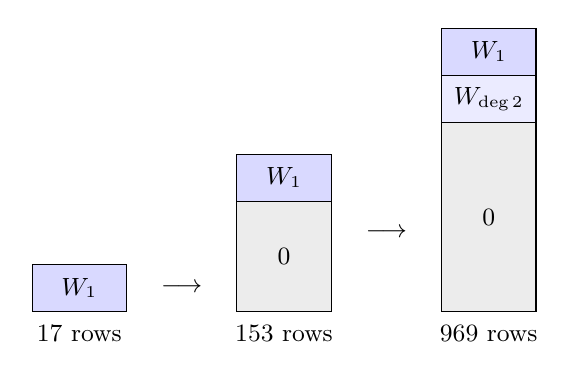
\begin{tikzpicture}[x=1cm,y=1cm,font=\small]
  % W1
  \draw[fill=blue!15] (0,0) rectangle (1.2,0.6);
  \node at (0.6,0.3) {$W_1$};
  \node[below] at (0.6,-0.05) {17 rows};
  \node at (1.9,0.3) {$\longrightarrow$};
  % W2
  \draw[fill=blue!15] (2.6,1.4) rectangle (3.8,2.0);
  \node at (3.2,1.7) {$W_1$};
  \draw[fill=gray!15] (2.6,0) rectangle (3.8,1.4);
  \node at (3.2,0.7) {$0$};
  \node[below] at (3.2,-0.05) {153 rows};
  \node at (4.5,1.0) {$\longrightarrow$};
  % W3
  \draw[fill=blue!15] (5.2,3.0) rectangle (6.4,3.6);
  \node at (5.8,3.3) {$W_1$};
  \draw[fill=blue!8] (5.2,2.4) rectangle (6.4,3.0);
  \node at (5.8,2.7) {$W_{\text{deg}\,2}$};
  \draw[fill=gray!15] (5.2,0) rectangle (6.4,2.4);
  \node at (5.8,1.2) {$0$};
  \node[below] at (5.8,-0.05) {969 rows};
\end{tikzpicture}
\caption{Zero-padding expansion (not to scale). The prefix structure of the feature map means the padded zero rows multiply the new, higher-degree features and contribute nothing to the old logits.}
\end{figure}

\subsection{Why zero initialization matters}

Before expansion the logits are $z_{\text{old}}(x)=\phi_1(x)^\top W_1$; after expansion $z_{\text{new}}(x)=\phi_2(x)^\top W_2$. Because the feature map is a prefix and the new weights are zero,
\[
\phi_2(x)^\top\begin{bmatrix}W_1\\0\end{bmatrix}=\phi_1(x)^\top W_1
\quad\Longrightarrow\quad
\boxed{z_{\text{new}}(x)=z_{\text{old}}(x)}.
\]
The softmax probabilities and predicted classes therefore remain unchanged too. This is an exact identity, subject only to floating-point rounding.

\begin{keybox}
The model gains new capacity without immediately changing its existing predictions.
\end{keybox}

\subsection{Does the package actually use expansion?}

Yes; it is part of the training loop. \code{run()} determines the active feature dimension from the schedule and grows the model when needed:
\begin{lstlisting}
count = int((deg <= DEGREES[t]).sum())
if count > len(W):
    probe = Phi_te[:64, :count]
    before = probe[:, :len(W)] @ W
    W = expand(W, count)
    assert np.allclose(probe @ W, before, atol=1e-9)
\end{lstlisting}
The model therefore goes $17\to153\to969$. The assertion checks logit preservation on a probe of 64 test examples; it is a diagnostic only, and test examples are never used for training.

\subsection{An important implementation distinction}

The complete degree-3 feature matrix is computed in \code{load\_digits\_features()} \emph{before} training starts, and the model is then shown the appropriate prefix. The package thus dynamically expands the \emph{trainable parameters and active feature dimension}, but it does not compute new features lazily. It demonstrates progressive model expansion, not reduced feature-computation cost.

%---------------------------------------------------------------------
\section{Degree-wise learning rates and degree control}

Instead of one scalar rate, each feature receives a rate set by its polynomial degree. With base rates $\eta=[\eta_0,\eta_1,\eta_2,\eta_3]\ (\ge0$, at least one positive) for the constant, degree-1, degree-2 and degree-3 groups, and \emph{degree-control factors} $m=[m_0,m_1,m_2,m_3]\in[0,1]^4$, the rate of feature $j$ is
\[
\boxed{d_j=\eta_{\deg(j)}\,m_{\deg(j)}},\qquad D=\diag(d),
\]
formed by \code{diagonal\_rates(eta, deg, control)}. Only the vector $d$ is built; $D$ is never formed. Ordinary SGD becomes
\[
\boxed{\Delta W=-DG},\qquad W_{\text{new}}=W_{\text{old}}-DG.
\]
This is a form of feature-group learning-rate control, and it follows the \code{diagonal\_control} PR of \code{polynomial\_cl}.

\subsection{Conventions enforced by the code}

All of the following are enforced by \code{diagonal\_rates} and tested in \code{tests/test\_degree\_control.py}: $m=\mathbf 1$ (or \code{control=None}) gives $d_j=\eta_{\deg(j)}$ exactly; $m_g=0$ freezes degree group $g$; an all-zero $d$ is a valid no-op experience; $\eta$ and $m$ must be real numbers (booleans, complex values and strings are rejected), finite, with $\eta\ge0$ and $m\in[0,1]$; and $m$ is never broadcast, so it must have exactly four entries. The map $j\mapsto d_j$ is \emph{prefix-stable}: a feature added by expansion takes the rate of its own degree, and old features keep theirs.

\subsection{Why is this useful?}

When the model expands from degree 1 to degree 2, the old degree-1 coefficients are already trained while the new degree-2 coefficients start at zero. One might choose a smaller factor for the old group, letting the new coefficients learn faster while making smaller changes to old ones. A factor $m_g=0$ freezes a group. This is a separate control from the null-space method: degree-wise rates control how strongly different feature groups participate in learning, while null-space optimization controls the \emph{direction} of the overall update relative to reference examples. The two combine through the metric $D$ that the null space is taken in.

\subsection{What does the current experiment use?}

The default experiment uses \code{eta = [3.0]*4} and no control ($m=\mathbf 1$), i.e.\ $d_j=3$ for every feature. The implementation \emph{supports} different rates and control factors, and \code{benchmark.py} studies single-degree control on validation data (\S\ref{sec:benchmark}), but the default demonstration does not assign different values to different degrees. This is the difference between a capability of the implementation and what the demonstration actually tests.

%=====================================================================
\part{Retained null-space continual learning}

\section{The central problem}

Replay gives the model old examples but does not guarantee that their predictions remain unchanged. For an old example $x_r$ with logits $z_r=\phi(x_r)^\top W$, ordinary SGD gives
\[
z_r^{\text{new}}-z_r=-\eta\,\phi(x_r)^\top G,
\]
which may be nonzero: gradients from new examples can change predictions on old ones. The package tries to prevent this by modifying the gradient \emph{direction}. The method is called \textbf{retained null-space continual learning}. Written out, its exact form is the \code{strategy\_b} step of the \code{polynomial\_cl} PR (project the gradient onto the null space of the reference inputs, in the metric of the diagonal rate); the package also keeps two \emph{relaxations} of it, named as such below.

%---------------------------------------------------------------------
\section{The reference matrix}

The method selects old replay examples as \emph{reference examples}. Let $R\in\R^{m\times p}$ be their feature matrix, one row $\phi(x_i)^\top$ per example. The package takes the first $n_{\text{ref}}$ stored examples of every old class: $n_{\text{ref}}=3$ for the exact \code{strategy\_b} step (the PR's default), and $n_{\text{ref}}=50$ for the relaxed variant. The reference matrix is built from replay features, never from held-out test data.

\begin{center}
\begin{tabular}{@{}ccccc@{}}
\toprule
Experience & Old classes & $m$ ($n_{\text{ref}}=50$) & Shape of $R$ & $n_{\text{ref}}=3$: shape of $R$\\
\midrule
2 & 0, 1 & 100 & $100\times153$ & $6\times153$\\
3 & 0--3 & 200 & $200\times969$ & $12\times969$\\
4 & 0--5 & 300 & $300\times969$ & $18\times969$\\
5 & 0--7 & 400 & $400\times969$ & $24\times969$\\
\bottomrule
\end{tabular}
\end{center}
Experience 1 has no old classes, hence no reference matrix.

For the current weights, the reference logits are $Z_{\text{ref}}=RW$. The goal is an update satisfying
\[
R\,\Delta W=0
\quad\Longrightarrow\quad
R(W+\Delta W)=RW,
\]
so the logits on the reference examples do not change. This is the mathematical retention constraint.

%---------------------------------------------------------------------
\section{What is a null space?}

The null space of a matrix $A$ is the set of vectors $v$ with $Av=0$. For $A=\begin{bmatrix}1&1\end{bmatrix}$ the vector $v=(1,-1)^\top$ belongs to it, since $Av=1-1=0$: one can move in this direction without changing the result of multiplying by $A$. That is the geometric idea of the method: find parameter-update directions that do not change the reference logits.

There is one complication. Because of the degree-wise learning rates, the package does not take the null space of $R$ itself, but of a \emph{rate-weighted} reference matrix.

%---------------------------------------------------------------------
\section{Incorporating degree-wise learning rates}

The package forms $A=RD^{1/2}$ and finds an orthonormal basis
\[
\boxed{N=\Null\!\bigl(RD^{1/2}\bigr)},\qquad RD^{1/2}N=0,\qquad N^\top N=I.
\]
It uses the singular value decomposition $RD^{1/2}=U\Sigma V^\top$. The right singular vectors whose singular values satisfy
\[
\sigma_i\le\text{tol}\cdot\max(\sigma_{\max},1)
\]
are treated as the null space. (The $\max(\sigma_{\max},1)$ is the \code{polynomial\_cl} convention; in the uncontrolled benchmark runs the smallest $\sigma_{\max}$ over splits and experiences is $4.59$, so there it equals $\sigma_{\max}$.) The default is $\text{tol}=10^{-10}$, which gives the exact null space up to rounding; the relaxed variant uses $\text{tol}=0.03$. For $\text{tol}=0.03$ this is a \textbf{numerical} null space, not the exact one, and as shown in \S\ref{sec:guarantee} the difference is large in practice. If there are no reference examples, $N=I$.

\subsection{Why use SVD?}

The singular values describe how strongly different directions affect the reference outputs: large values mean a direction changes them substantially, small values weakly, and directions treated as zero form the numerical null space. The number of retained null-space directions depends on the feature dimension, the reference examples, the learning rates, and the tolerance.

%---------------------------------------------------------------------
\section{Projecting the gradient}

We have the gradient $G$, the rate matrix $D$, and the null-space basis $N$. First scale the gradient, $G_s=D^{1/2}G$, then project it: $G_{\text{null}}=NN^\top G_s$. Because $N^\top N=I$, the matrix $P=NN^\top$ is the orthogonal projector onto the null space, and for an exact null space
\[
RD^{1/2}G_{\text{null}}=0.
\]
Using only this projected gradient would preserve the reference logits for that update. The trade-off is that useful learning directions may lie \emph{outside} the null space, and removing them can severely limit plasticity. The package therefore introduces a parameter $\beta$.

%---------------------------------------------------------------------
\section{The role of beta: balancing retention and learning}

The central update equation is
\[
\boxed{\Delta W=-D^{1/2}\Bigl[NN^\top+\beta\,(I-NN^\top)\Bigr]D^{1/2}G},\qquad 0\le\beta\le1.
\]
Writing $G_s=PG_s+(I-P)G_s$, the update is $-D^{1/2}[PG_s+\beta(I-P)G_s]$: the null-space component receives its full update, and the orthogonal component only a fraction $\beta$.

\begin{figure}[h]
\centering
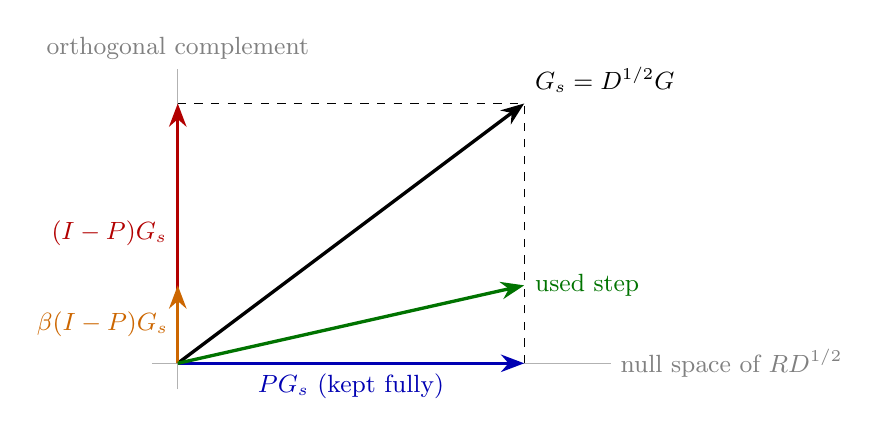
\begin{tikzpicture}[scale=1.1,>=Stealth,font=\small]
  % axes
  \draw[gray!60] (-0.3,0) -- (5,0);
  \draw[gray!60] (0,-0.3) -- (0,3.4);
  \node[gray,right] at (5,0) {null space of $RD^{1/2}$};
  \node[gray,above] at (0,3.4) {orthogonal complement};
  % G_s
  \draw[very thick,->] (0,0) -- (4,3) node[above right] {$G_s=D^{1/2}G$};
  \draw[dashed] (4,0) -- (4,3);
  \draw[dashed] (0,3) -- (4,3);
  % components
  \draw[very thick,blue!70!black,->] (0,0) -- (4,0) node[midway,below] {$PG_s$ (kept fully)};
  \draw[very thick,red!70!black,->] (0,0) -- (0,3) node[midway,left] {$(I-P)G_s$};
  \draw[very thick,orange!80!black,->] (0,0) -- (0,0.9) ;
  \node[orange!80!black,left] at (0,0.45) {$\beta(I-P)G_s$};
  % resulting
  \draw[very thick,green!45!black,->] (0,0) -- (4,0.9) node[right] {used step};
\end{tikzpicture}
\caption{Geometry of the update for $\beta=0.3$. The component in the null space (blue) is kept; the orthogonal component (red) is shrunk to a fraction $\beta$ (orange); the used step (green) is their sum. With $\beta=0$ the used step lies on the horizontal axis; with $\beta=1$ it is the full $G_s$.}
\end{figure}

\subsection{Beta equals zero}

$\Delta W=-D^{1/2}NN^\top D^{1/2}G$. Only the null-space component is used, and with an exact null space $\boxed{R\Delta W=0}$: the reference logits are preserved for that step, at the possible cost of learning ability.

\subsection{Beta equals one}

Since $NN^\top+(I-NN^\top)=I$, we get $\Delta W=-DG$, which is ordinary degree-wise SGD:
\[
\boxed{\beta=1\ \Longrightarrow\ \text{ordinary SGD}}.
\]

\subsection{Intermediate beta}

For $0<\beta<1$ the method retains the full null-space component but allows a reduced amount of the orthogonal component. With $\beta=0.3$ (the relaxed variant), 30\% of the orthogonal component passes through. The exact \code{strategy\_b} step uses $\beta=0$. This is not a simple reduction of the whole learning rate; it changes the \emph{direction} of the update by treating two geometrically different components differently. That is why the method is more than conventional learning-rate reduction---or at least, that is the hypothesis the benchmark tests (\S\ref{sec:benchmark}).

%---------------------------------------------------------------------
\section{What does the null-space update actually guarantee?}\label{sec:guarantee}

Define $E=RD^{1/2}N$, which is zero for an exact null space. Expanding the update,
\[
\boxed{R\Delta W=-(1-\beta)\,E\,N^\top D^{1/2}G-\beta\,RDG.}
\]
For an exact null space $E=0$ and
\[
\boxed{R\Delta W=-\beta\,RDG}.
\]
\begin{center}
\begin{tabular}{@{}cl@{}}
\toprule
$\beta$ & Reference-logit behaviour\\
\midrule
0 & No per-step reference-logit change\\
0.3 & Generally permits some reference-logit change\\
1 & Same change as ordinary degree-wise SGD\\
\bottomrule
\end{tabular}
\end{center}
A nonzero $\beta$ \emph{permits} drift but does not necessarily \emph{cause} it: if $RDG=0$, then $R\Delta W=0$ even for $\beta>0$. It would therefore be wrong to say that every update with $\beta>0$ must damage reference predictions.

\subsection{What happens with numerical tolerance?}

With $\text{tol}=0.03$, directions with small but nonzero singular values are treated as null, so in general $E\neq0$, and even with $\beta=0$ the reference-logit change is not exactly zero. The method gives \emph{approximate} per-step retention, not an unconditional guarantee.

\begin{verifybox}
How approximate? On split 0 with $\eta=3$, the singular values of $RD^{1/2}$ have exact rank 100, 200, 300, 400 at experiences 2--5, but a threshold of $0.03\,\sigma_{\max}$ (here $\sigma_{\max}>1$) keeps only 45, 54, 38, 52 of them. The numerical ``null space'' therefore contains many directions that do affect the reference logits (Appendix~\ref{app:verify}). In a test with a random gradient at experience 5 and $\beta=0$, the reference-logit change was about $10.6\%$ of what ordinary SGD would cause, versus $\sim10^{-15}$ when $\text{tol}=10^{-10}$. In practice the method protects the \emph{dominant} reference directions and shrinks, rather than eliminates, the rest.
\end{verifybox}

\subsection{What the step provably does}

Write $u=D^{1/2}G$, $P=NN^\top$, $S=\{j:d_j>0\}$, and let $R_S$ keep the columns of $R$ in $S$. For the \emph{exact} step ($\beta=0$, $\text{tol}\to0$, so $P$ projects onto $\Null(RD^{1/2})$), \code{math.tex} proves:
\begin{enumerate}[label=(\alph*)]
\item $R\,\Delta W=0$: every reference logit is unchanged after each step.
\item Row $j$ of $\Delta W$ is zero whenever $d_j=0$, so a frozen degree group does not move.
\item $\Delta W$ is the unique minimiser of $\langle G,Z\rangle+\tfrac12\sum_{j\in S}\|Z_j\|^2/d_j$ over updates $Z$ with $Z_{S^c}=0$ and $RZ=0$: the best descent step that cannot move the reference logits.
\item $\langle G,\Delta W\rangle=-\|Pu\|_F^2\le0$, and the step stalls ($\Delta W=0$) exactly when $Pu=0$.
\item Only $r=\operatorname{rank}(D^{1/2}N)=|S|-\operatorname{rank}(R_S)$ directions are free to move (\code{free\_dim}); $r=0$ means no learning at all.
\end{enumerate}
For the \emph{relaxation} (any $\beta,\text{tol}$, with $\tau=\text{tol}\cdot\max(\sigma_{\max},1)$): $\beta=1$ is ordinary SGD; $\langle G,\Delta W\rangle=-\bigl(\beta\|u\|_F^2+(1-\beta)\|Pu\|_F^2\bigr)\le0$, so every step is non-ascent; and
\[
\bigl\|R\,\Delta W+\beta\,RDG\bigr\|_F\le(1-\beta)\,\tau\,\|D^{1/2}G\|_F,
\]
i.e.\ reference logits move by $\beta$ times their SGD change, up to a term proportional to the tolerance. All of these identities hold on the reference matrix only.

\begin{verifybox}
Free dimension. With all four rates positive, $\operatorname{rank}(R_S)=\operatorname{rank}(R)$, so the number of free directions equals the null-space dimension. For the exact step with $n_{\text{ref}}=3$ ($\eta=3$, split 0, memory 100, seed 3) it is $147,957,951,945$ at experiences 2--5, out of $153,969,969,969$ features; with $n_{\text{ref}}=50$ it is $53,769,669,569$ (Appendix~\ref{app:verify}). The \emph{number} of constraints is therefore small for $n_{\text{ref}}=3$, yet the measured cost of the exact step is high (\S\ref{sec:benchmark}): a small number of constraints does not mean little lost learning.
\end{verifybox}

\subsection{Per-step retention versus accumulated drift}

Small per-step changes can accumulate over many minibatches. We must therefore distinguish: (1)~per-step reference-logit preservation; (2)~accumulated reference-logit drift over an experience; (3)~classification accuracy on old replay examples; and (4)~classification accuracy on held-out old test examples. These are different quantities. A small per-step change does not guarantee low accumulated drift, and preserving reference logits does not guarantee unchanged held-out accuracy. This is an important limitation.

%---------------------------------------------------------------------
\section{How expansion interacts with null-space optimization}

Suppose the model starts at degree 1 ($W_1\in\R^{17\times10}$), trains on experience 1, and at experience 2 expands to $W_2=\begin{bmatrix}W_1\\0\end{bmatrix}$. Old predictions are preserved at the moment of expansion. But a null-space basis built for the previous feature dimension cannot simply be reused. The package therefore reconstructs the basis inside \code{train\_task()} for the current feature space and current reference matrix, \emph{once per experience} (the basis is then held fixed across that experience's epochs and minibatches).

\subsection{Why rebuild the basis?}

After expansion the reference matrix has additional columns, $R_2\in\R^{m\times153}$, and the basis must correspond to $N_2=\Null(R_2D_2^{1/2})$. If the old basis were merely zero-padded, the new coordinates would have no active directions in it, so at $\beta=0$ the new coefficients could not learn at all. Rebuilding solves this.

\subsection{The complete sequence}

\begin{enumerate}
\item Train on the current experience.
\item When the next experience arrives, expand the feature dimension if necessary.
\item Initialize the new coefficient rows to zero.
\item Preserve existing logits at expansion.
\item Select replay examples from previous classes.
\item Rebuild the null-space basis for the current feature dimension.
\item Train using ordinary SGD or the retained null-space update.
\item Evaluate all classes learned so far.
\end{enumerate}
The two mechanisms have separate responsibilities: expansion preserves predictions at the instant capacity increases; null-space optimization attempts to preserve them during subsequent training. Neither replaces the other.

%=====================================================================
\part{The actual training and evaluation process}

\section{What happens during an experiment}

\code{run()} begins with $W\in\R^{17\times10}$, all zeros, and a fixed replay memory of 100 training examples per class. Then:

\paragraph{Experience 1 --- digits 0 and 1.} Features $\phi_1(x)\in\R^{17}$; only the first two output columns are used. There are no old classes, so there is no replay memory, and even if null-space optimization is selected, experience 1 uses ordinary SGD because there are no reference examples. Three epochs, then evaluation on test digits 0 and 1.

\paragraph{Experience 2 --- digits 2 and 3.} Degree $1\to2$, features $17\to153$, $W_2=\begin{bmatrix}W_1\\0\end{bmatrix}$, four output columns. Training data: current digits 2, 3 plus replay of 0, 1. With null-space selected, the reference matrix is built from old replay examples and a new basis is computed. Evaluation on digits 0--3.

\paragraph{Experience 3 --- digits 4 and 5.} Degree $2\to3$, features $153\to969$, new rows zero, six output columns. Training data: digits 4, 5 plus replay of 0--3. Basis rebuilt in the new space. Evaluation on digits 0--5.

\paragraph{Experience 4 --- digits 6 and 7.} Degree stays 3 ($969\to969$, no expansion), eight output columns; current digits 6, 7 plus replay of 0--5. Evaluation on digits 0--7.

\paragraph{Experience 5 --- digits 8 and 9.} Degree 3 again, all ten output columns; current digits 8, 9 plus replay of 0--7. Evaluation on all ten classes.

\begin{center}
\begin{tabular}{@{}cccccc@{}}
\toprule
Exp. & New classes & Features & Active classes & Training data & Null-space used?\\
\midrule
1 & 0, 1 & 17 & 2 & Current & no (no reference)\\
2 & 2, 3 & 153 & 4 & Current + replay & yes\\
3 & 4, 5 & 969 & 6 & Current + replay & yes\\
4 & 6, 7 & 969 & 8 & Current + replay & yes\\
5 & 8, 9 & 969 & 10 & Current + replay & yes\\
\bottomrule
\end{tabular}
\end{center}
This is the actual progressive class-incremental experiment implemented by the package.

%---------------------------------------------------------------------
\section{What exactly does the package measure?}

The package records performance after \emph{every} experience, giving a lower-triangular accuracy matrix $A\in\R^{5\times5}$ where $A_{t,j}$ is the accuracy on experience $j$'s test examples after training experience $t$:
\[
A=\begin{bmatrix}
A_{1,1}&-&-&-&-\\
A_{2,1}&A_{2,2}&-&-&-\\
A_{3,1}&A_{3,2}&A_{3,3}&-&-\\
A_{4,1}&A_{4,2}&A_{4,3}&A_{4,4}&-\\
A_{5,1}&A_{5,2}&A_{5,3}&A_{5,4}&A_{5,5}
\end{bmatrix}.
\]
The diagonal is performance immediately after learning each experience; the last row is performance after the whole sequence. Five metrics are derived.

\subsection{Final accuracy}
\[
\text{Accuracy}=\frac15\sum_{j=1}^{5}A_{5,j}.
\]
The main overall metric: average final accuracy across the five class groups.

\subsection{Forgetting}
For each of the first four experiences, the best accuracy it reached up to experience 4 is compared with its final accuracy:
\[
F_j=\max_{t=j,\ldots,4}A_{t,j}-A_{5,j},
\qquad
\boxed{F=\frac14\sum_{j=1}^{4}F_j}.
\]
The fifth experience is excluded because nothing follows it. Lower is better.

\subsection{Plasticity}
\[
\boxed{P=\frac15\sum_{j=1}^{5}A_{j,j}}.
\]
Immediate learning performance on each new experience. Particularly important, because low forgetting can come from a model that simply refuses to learn.

\subsection{Newest-experience accuracy}
\[
\boxed{A_{\text{newest}}=A_{5,5}}.
\]
How well the model handles the latest classes at the end of the sequence, a check that it can still learn.

\subsection{Old-experience accuracy}
\[
\boxed{A_{\text{old}}=\frac14\sum_{j=1}^{4}A_{5,j}}.
\]
Final accuracy on the first four experiences: how well old classes are retained.

\begin{keybox}[title={Read the metrics together}]
A model with low forgetting but very poor newest-experience accuracy is not necessarily a good continual learner.
\end{keybox}

%=====================================================================
\part{The experiments and what they establish}

\section{Ordinary SGD versus the null-space update}\label{sec:demo}

\textbf{Method A --- ordinary SGD:} $\Delta W=-DG$. The baseline; it learns with the diagonal rates but no explicit constraint relative to reference examples.

\textbf{Method B --- exact \code{strategy\_b}:} $\Delta W=-D^{1/2}\bigl[NN^\top+\beta(I-NN^\top)\bigr]D^{1/2}G$ with $\beta=0$, $\text{tol}=10^{-10}$, $n_{\text{ref}}=3$ (the PR's defaults). It tries to leave old reference logits unchanged.

\textbf{Method C --- relaxed null-space update:} the same formula with $\text{tol}=0.03$, $\beta=0.3$, $n_{\text{ref}}=50$. A spectral tolerance and a blend toward ordinary SGD are the two relaxations; they are not \code{strategy\_b}, they are what the earlier package tuned.

The \code{demo()} function compares them with: data split seed 0; training seeds 3, 4, 5, 6, 7; 100 replay examples per class; three epochs per experience; learning rate 3 for every degree and no degree control.

\begin{verifybox}
Running \code{python -m stable\_cl} reproduces:
\begin{center}\small
\begin{tabular}{@{}lccccc@{}}
\toprule
Method & Accuracy & Forgetting & Plasticity & Newest & Old\\
\midrule
Ordinary SGD & 0.813 & 0.052 & 0.840 & 0.653 & 0.852\\
Exact \code{strategy\_b} & 0.777 & 0.029 & 0.790 & 0.391 & 0.873\\
Relaxed ($\text{tol}=.03$, $\beta=.3$, $n_{\text{ref}}=50$) & 0.831 & 0.033 & 0.838 & 0.647 & 0.878\\
\bottomrule
\end{tabular}
\end{center}
The exact step has the lowest forgetting, but it pays for it with plasticity (0.790 vs.\ 0.840) and newest-experience accuracy (0.391 vs.\ 0.653): its low forgetting is partly a failure to learn. The relaxed step keeps plasticity essentially unchanged (0.838) while forgetting falls and old-class accuracy rises. This is one data split with five training seeds, so it is a demonstration, not a significance test.
\end{verifybox}

\section{What does \texttt{benchmark.py} investigate?}\label{sec:benchmark}

The benchmark asks the harder question: if a null-space update forgets less, is that because its geometric update is useful, or simply because it effectively \emph{reduces learning}? It therefore compares against ordinary SGD with learning-rate multipliers $1.0,\,0.75,\,0.5,\,0.35,\,0.25$, and it reports the exact \code{strategy\_b} step next to the relaxation, so the cost of the exact step is visible.

\subsection{Validation}

Only the relaxation is tuned. It tries $\text{tol}\in\{0.3,0.1,0.03,0.01\}$ and $\beta\in\{0,0.1,0.3\}$, with $n_{\text{ref}}=50$, on four validation splits (seeds 100--103) with two training seeds and memory 60 per class. (A memory of 100 per class is not available on every validation split: even after stratification split 103 has only 96 fitting examples of digit 8, and \code{run()} then raises an explicit error instead of resampling with replacement.) Among configurations satisfying a \emph{predeclared} requirement
\[
F_{\text{null}}\le0.7\,F_{\text{ordinary}},
\]
(at least 30\% less forgetting on validation data) it selects the one with the highest validation accuracy, and raises an error if none qualifies. Test data is not used for this selection. The selected configuration is $\text{tol}=0.03$, $\beta=0.3$ (ordinary validation forgetting $0.053$).

\subsection{Testing}

The exact step and the selected relaxation are compared with ordinary SGD and the learning-rate controls over ten test splits, two training seeds per split, and memory sizes 60 and 100. The benchmark computes paired 95\% confidence intervals (a $t$-interval over the ten split-level differences) for accuracy and forgetting for three comparisons (exact vs.\ ordinary, relaxed vs.\ ordinary, relaxed vs.\ exact), and compares the relaxation with the measured smaller-learning-rate frontier. The relaxation is declared to have ``value'' if the lower accuracy bound exceeds $-0.01$ (non-inferiority) and the upper forgetting bound is below 0.

\subsection{Reported results}

All numbers are printed by \code{benchmark.py} (Appendix~\ref{app:verify}); differences are first minus second method, with 95\% intervals:
\begin{center}\scriptsize\setlength{\tabcolsep}{3pt}
\begin{tabular}{@{}llcc@{}}
\toprule
Memory & Comparison & $\Delta A$ [95\% CI] & $\Delta F$ [95\% CI]\\
\midrule
60 & exact $-$ ordinary & $-0.048\,[-0.059,-0.037]$ & $-0.022\,[-0.030,-0.014]$\\
60 & relaxed $-$ ordinary & $-0.003\,[-0.012,+0.006]$ & $-0.022\,[-0.034,-0.011]$\\
60 & relaxed $-$ exact & $+0.045\,[+0.031,+0.058]$ & $-0.000\,[-0.008,+0.008]$\\
100 & exact $-$ ordinary & $-0.030\,[-0.040,-0.020]$ & $-0.015\,[-0.022,-0.007]$\\
100 & relaxed $-$ ordinary & $+0.003\,[-0.003,+0.009]$ & $-0.019\,[-0.026,-0.012]$\\
100 & relaxed $-$ exact & $+0.033\,[+0.021,+0.046]$ & $-0.004\,[-0.016,+0.007]$\\
\bottomrule
\end{tabular}
\end{center}
Exact \code{strategy\_b} lowers forgetting but also newest-experience accuracy (0.227 vs.\ 0.515 at memory 60; 0.334 vs.\ 0.559 at memory 100). At memory 60 the relaxation's lower accuracy bound ($-0.012$) just misses the $-0.01$ requirement, so \code{benchmark.py} prints ``no value'' there (frontier margin $+0.041$) even though forgetting falls significantly; at memory 100 the criterion is met (``VALUE'') and the relaxation also exceeds the learning-rate frontier ($+0.058$).

\subsection{Degree control}

The benchmark also applies the PR's degree-control selection rule, for single-degree candidates only, on top of each base update. Candidates are $m=\mathbf 1$ plus each single degree set to one factor in $\{0,.05,.1,.25,.5,.75\}$ (25 in all). On validation data a candidate is \emph{feasible} if the mean accuracy right after each experience, taken over seeds and splits, is at least the acquisition floor $0.5$ for every experience; formally $\min_t\overline{A_{t,t}}\ge0.5$ with the bar a mean over seeds \emph{and} splits, so the minimum is taken after averaging, not within each split. Among feasible candidates the rule keeps the Pareto front of (accuracy, forgetting), then takes the largest accuracy minus forgetting; if none is feasible, nothing is selected. Test data never enters selection.

\begin{center}\small
\begin{tabular}{@{}lccp{6.6cm}@{}}
\toprule
Base update & Feasible (of 25) & Selected & Test effect at memory 60\\
\midrule
ordinary SGD & 13 & $m=[1,0.1,1,1]$ & $\Delta A=-0.004\,[-0.019,+0.010]$, $\Delta F=-0.006\,[-0.018,+0.007]$; smallest mean arrival accuracy $0.515\to0.490$\\
exact \code{strategy\_b} & 0 & none & ---\\
relaxed update & 0 & none & ---\\
\bottomrule
\end{tabular}
\end{center}
For ordinary SGD the selected control changes accuracy by an amount indistinguishable from zero, and its forgetting change ($-0.006$) is also indistinguishable from zero: its interval contains $0$. On the test splits the smallest mean arrival accuracy falls from 0.515 to 0.490, below the floor $0.5$ that was satisfied on validation data. So this experiment gives \emph{no evidence} that degree control lowers forgetting. An earlier validation protocol (unstratified cut) selected $m=[1,0,1,1]$ and showed $\Delta F=-0.027\,[-0.041,-0.013]$; that result did not survive stratifying the validation splits, i.e.\ the apparent benefit depended on which candidate a small, noisy validation set happened to select. It should not be quoted as a finding. For the exact step and for the relaxed variant \emph{no} candidate is feasible (0 of 25); by the rule nothing is selected, so no test comparison is made. The acquisition floor was set with Split MNIST in view and was not tuned for digits; for the exact step no candidate is feasible because even the all-ones baseline stays below the floor on some experience. The PR's combination step and Split-MNIST study are not repeated here.

\begin{reviewbox}
How strong is this evidence? Four honest qualifications. (i)~The relaxation's accuracy intervals contain zero at both memory sizes: the result is ``no measurable accuracy loss with less forgetting'', not ``better accuracy''. (ii)~The exact \code{strategy\_b} step, the one with the logit-preservation guarantee, is clearly worse than ordinary SGD in accuracy at both memory sizes; the practical value sits in the relaxation, which is exactly the part the guarantee does not cover. (iii)~The frontier margin is the relaxation's accuracy minus the accuracy that \code{np.interp} reads off the learning-rate curve at the same forgetting; \code{np.interp} clamps outside the range of the learning-rate controls rather than extrapolating. The verdict rule itself uses only the accuracy and forgetting intervals, not the frontier margin. (iv)~All of it concerns one small dataset, one fixed random projection, and one five-experience protocol. The result is encouraging evidence that the relaxed geometric update offers something beyond lowering the learning rate, but it is not conclusive.
\end{reviewbox}

%=====================================================================
\part{The complete package architecture}

\section{What does each file do?}

The package consists of the following files. The PDFs of the two \LaTeX{} documents are \emph{not} committed; they are built locally (see \code{README.md}).

\begin{center}
\begin{tabular}{@{}lp{9.6cm}@{}}
\toprule
File & Responsibility\\
\midrule
\code{stable\_cl/features.py} & Polynomial feature map and zero-initialized expansion.\\
\code{stable\_cl/optimization.py} & Diagonal degree-wise rates, the null-space basis, the (relaxed) null-space step and the free dimension.\\
\code{stable\_cl/training.py} & Softmax and the training of one experience on current data plus replay.\\
\code{stable\_cl/experiment.py} & Data preparation, the five class-incremental experiences, the metrics and the demo.\\
\code{benchmark.py} & Validation-based selection of the relaxation, comparisons against ordinary SGD, smaller learning rates and the exact step, and the degree-control study.\\
\code{tests/} & The pytest suite that checks the mathematical properties of every function.\\
\code{README.md} & Short description, run and build instructions.\\
\code{math.tex} & LaTeX source of the mathematical specification: definitions, propositions, proofs, results.\\
\code{explain.tex} & LaTeX source of this document.\\
\bottomrule
\end{tabular}
\end{center}

The key functions are:

\begin{center}
\begin{tabular}{@{}llp{8.2cm}@{}}
\toprule
Function & Module & Responsibility\\
\midrule
\code{poly\_features()} & \code{features} & Generates degree-ordered, degree-scaled polynomial features.\\
\code{expand()} & \code{features} & Adds zero-initialized coefficient rows.\\
\code{diagonal\_rates()} & \code{optimization} & Builds and validates the vector $d_j=\eta_{\deg(j)}m_{\deg(j)}$.\\
\code{null\_basis()} & \code{optimization} & Computes the numerical null-space basis of $RD^{1/2}$ by SVD.\\
\code{null\_step()} & \code{optimization} & Computes the rate-weighted null-space step (returned unsigned; $\Delta W$ is its negative).\\
\code{free\_dim()} & \code{optimization} & Counts the feature directions that can still move, $\operatorname{rank}(D^{1/2}N)$.\\
\code{softmax()} & \code{training} & Converts logits into probabilities.\\
\code{train\_task()} & \code{training} & Trains one experience on current data plus replay, with \code{strategy}, \code{control}, \code{n\_ref}, \code{tol}, \code{beta}.\\
\code{run()} & \code{experiment} & Runs all five experiences and computes the metrics.\\
\code{load\_digits\_features()} & \code{experiment} & Loads, splits, standardises (fitting-set statistics), projects and transforms the digits dataset.\\
\code{stratified\_cut()} & \code{experiment} & Splits indices so that every class keeps $\lfloor f\,n_c\rfloor$ examples in the first part (used for the validation cut).\\
\code{demo()} & \code{experiment} & Runs the ordinary / exact / relaxed demonstration (\code{CONFIGS}).\\
\bottomrule
\end{tabular}
\end{center}

Every function carries a docstring stating its purpose, argument shapes, return value and, where it implements a mathematical operation, the same equation as in this document and in \code{math.tex}.

The benchmark calls \code{run()} rather than implementing a second training algorithm, so the demonstration and the benchmark exercise the same learning system. This is good design.

\section{What has deliberately been removed?}

The package retains two update families: ordinary SGD and the rate-weighted null-space update. The earlier margin-based per-step and cumulative task-budget $\alpha$-gates were removed. According to the package's specification they either suppressed learning or reduced accuracy too much to be useful in the supplied benchmark. (Those experiments are not included in the package, so this explanation cannot independently confirm that conclusion.) What the current version \emph{adds} is the PR's diagonal degree control and the name \code{strategy\_b} for the exact step; the spectral tolerance and the blend $\beta$ are kept as named relaxations of it.

%=====================================================================
\part{What the package proves, and what it does not}

\section{What is mathematically established?}

\begin{enumerate}
\item \textbf{Polynomial feature prefix property.} Lower-degree features are prefixes of higher-degree feature maps.
\item \textbf{Expansion invariance.} Appending zero rows preserves logits: $\phi_{d+1}(x)^\top\begin{bmatrix}W_d\\0\end{bmatrix}=\phi_d(x)^\top W_d$.
\item \textbf{Diagonal-rate conventions.} $m=\mathbf 1$ is the uncontrolled rate, $m_g=0$ freezes a group, an all-zero rate is a no-op, and the rate map is prefix-stable.
\item \textbf{Exact null-space step.} For $\beta=0$ and exact null space: $R\Delta W=0$, frozen rows stay fixed, the step is the constrained minimiser of Proposition~1(c) of \code{math.tex}, and it is a descent step.
\item \textbf{Ordinary-SGD equivalence.} At $\beta=1$: $\Delta W=-DG$ for every tolerance.
\item \textbf{Relaxation bound.} For any $\beta,\text{tol}$ the reference logits move by $\beta$ times their SGD change up to $(1-\beta)\,\text{tol}\cdot\max(\sigma_{\max},1)\,\|D^{1/2}G\|_F$, and every step is non-ascent.
\item \textbf{Compatibility.} The model can expand, rebuild the null-space basis, and continue learning the new coefficients.
\end{enumerate}
These are properties of the implementation and its mathematical construction. The pytest suite (\code{tests/}) tests the polynomial feature count, ordering and prefix property, expansion invariance, the diagonal-rate conventions, the exact step ($R\Delta W=0$, frozen rows, an independent pseudo-inverse form, the constrained-minimiser property, the free dimension), the endpoint $\beta=1$, the blend identity and the relaxation bound on random data, the cross-entropy gradient inside \code{train\_task} against finite differences, whole-experience reference-logit invariance on toy data, that an all-ones control reproduces the uncontrolled run and an all-zero control is a no-op, the metric definitions, that evaluation rows do not influence preprocessing, the benchmark statistics and selection rule, and (when \code{polynomial\_cl} is importable) one step against the PR. The exact-step properties use an \emph{exact} null space ($\text{tol}\approx10^{-10}$); they do not carry over to the relaxed $\text{tol}=0.03$ except through the bound above. In the environment used for Appendix~\ref{app:verify} \code{polynomial\_cl} was not installed, so the PR-parity test was skipped.

\section{What has not been established?}

\begin{itemize}
\item The experiments use one small handwritten-digit dataset.
\item The model uses one fixed random projection.
\item Only five experiences are tested.
\item The default demonstration uses the same learning rate for all degrees; degree control is studied only for single-degree candidates, with a floor set for another dataset.
\item Only a small grid of null-space hyperparameters is explored.
\item The benefit of the relaxed update is empirical and outside the logit-preservation guarantee of the exact step.
\item Numerical reference-logit preservation does not guarantee preservation of held-out accuracy.
\item Nothing is shown about generalization to other datasets.
\item No computational or memory advantage of progressive expansion is demonstrated.
\item No expansion schedules are compared with one another.
\item The PR's combination step and Split-MNIST study are not repeated, and agreement with \code{polynomial\_cl} was not tested in the verification environment.
\end{itemize}
That gap deserves emphasis:

\begin{keybox}[title={An important gap}]
The package uses progressive expansion in its actual experiments, but it does not include an ablation comparing progressive expansion against fixed degree~1 or fixed degree~3. Its benchmark isolates the value of the null-space update against ordinary SGD and smaller learning rates, \emph{under the same expansion schedule}.
\end{keybox}

%=====================================================================
\section{Final conceptual picture}\label{sec:final}

The complete system can be understood as three interacting layers:

\begin{figure}[h]
\centering
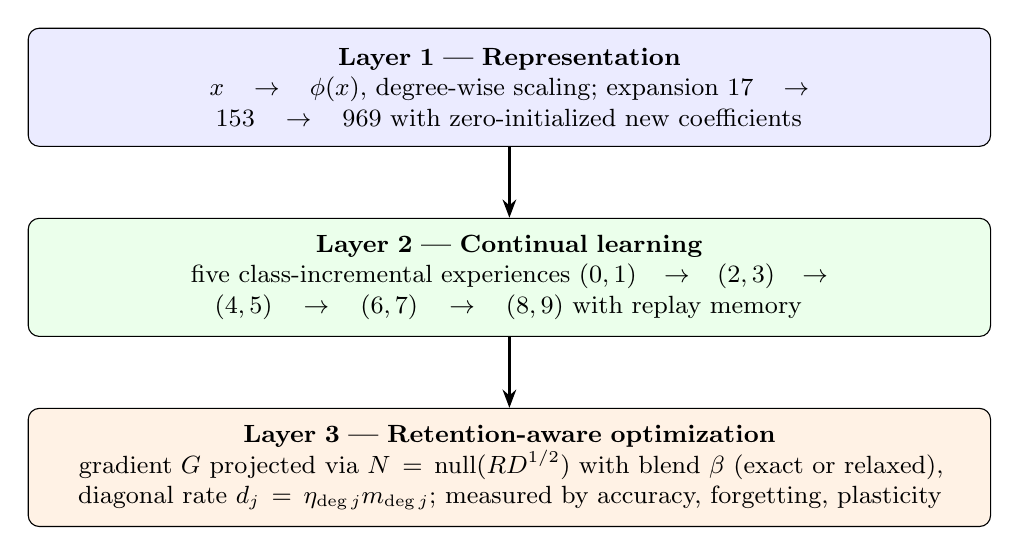
\begin{tikzpicture}[node distance=0.9cm,>=Stealth,font=\small,
  layer/.style={draw,rounded corners,align=center,text width=11.8cm,minimum height=1.5cm,inner sep=6pt}]
  \node[layer,fill=blue!8] (l1) {\textbf{Layer 1 --- Representation}\\
    $x\to\phi(x)$, degree-wise scaling; expansion $17\to153\to969$ with zero-initialized new coefficients};
  \node[layer,fill=green!8,below=of l1] (l2) {\textbf{Layer 2 --- Continual learning}\\
    five class-incremental experiences $(0,1)\to(2,3)\to(4,5)\to(6,7)\to(8,9)$ with replay memory};
  \node[layer,fill=orange!10,below=of l2] (l3) {\textbf{Layer 3 --- Retention-aware optimization}\\
    gradient $G$ projected via $N=\Null(RD^{1/2})$ with blend $\beta$ (exact or relaxed), diagonal rate $d_j=\eta_{\deg j}m_{\deg j}$; measured by accuracy, forgetting, plasticity};
  \draw[->,thick] (l1) -- (l2);
  \draw[->,thick] (l2) -- (l3);
\end{tikzpicture}
\caption{The three layers of the package.}\label{fig:layers}
\end{figure}

\paragraph{Layer 1 --- Representation.} The polynomial transformation $x\longrightarrow\phi(x)$ creates the feature space; progressive expansion increases its dimension $17\to153\to969$, and new coefficients start at zero, preserving existing predictions.

\paragraph{Layer 2 --- Continual learning.} The classifier receives new classes sequentially, and replay memory brings selected old examples back into training.

\paragraph{Layer 3 --- Retention-aware optimization.} The model computes the cross-entropy gradient $G$ and modifies it using the null-space basis $N=\Null(RD^{1/2})$ of the diagonally rate-weighted reference matrix, exactly (\code{strategy\_b}) or in relaxed form. The update tries to learn new information while reducing changes to predictions on selected replay examples. Finally the package measures accuracy, forgetting, plasticity, newest accuracy, and old accuracy.

\section{The central idea in one paragraph}

The package implements a class-incremental polynomial classifier that starts with a small feature representation and progressively expands its trainable polynomial dimensions as new classes arrive. New coefficients are initialized to zero, so expansion itself does not change existing predictions. During each subsequent experience, the model trains on new examples together with replay examples from earlier classes. Ordinary SGD is the baseline, while the null-space update modifies the gradient using the null space of the rate-weighted replay feature matrix: exactly, as \code{strategy\_b}, which preserves reference logits but learns little, or in a relaxed form with a spectral tolerance and a blend toward SGD, which is what keeps plasticity. This encourages updates that preserve predictions on selected old examples while allowing learning in other directions. The system evaluates the balance between plasticity and retention across five sequential class experiences.

\paragraph{Overall interpretation.} The interesting contribution is not polynomial expansion, replay, or gradient projection in isolation, but their combination: an expandable polynomial representation with degree-wise learning-rate control and a geometrically constrained update rule, tested in a class-incremental setting. The honest status is a modest, well-controlled result on one small benchmark, and it belongs to the relaxed update rather than to the exact step that carries the guarantee.

%=====================================================================
\appendix
\section{Corrections and changes}\label{app:corrections}

\subsection{Corrections made relative to the original \texttt{explain.md}}

These corrections were made in the previous edition of this document and are kept.

\begin{enumerate}
\item \textbf{Matrix shapes (\S12 of the original).} The original illustrated experience 3 (reference examples from digits 0--3, $m=200$) with $R\in\R^{200\times153}$. At experience 3 the model already has 969 features, so the correct shape is $200\times969$ (and experience 2 gives $100\times153$). A full table is included.
\item \textbf{Missing diagram.} The final ``three interacting layers'' picture in the original was blank; it is drawn (Figure~\ref{fig:layers} in \S\ref{sec:final}).
\item \textbf{Numerical tolerance understated.} The original said only that the null space is numerical and ``$E\neq0$ in general''. Running the code shows the tolerance of 0.03 is a large approximation (Appendix~\ref{app:verify}): it protects only the 38--54 dominant reference directions, not all 100--400. The text says so.
\item \textbf{Basis rebuilt once per experience.} The basis is computed once at the start of each \code{train\_task()} call, not per minibatch.
\item \textbf{Unscaled illustration.} The two-dimensional polynomial example omits the degree scaling; this is stated.
\item \textbf{Strength of the benchmark claim.} The original called the result ``useful evidence'' that geometry beats lowering the learning rate. The qualifications (zero-containing accuracy intervals, clamped interpolation, one dataset) are stated explicitly.
\item \textbf{First-person remark.} ``My overall interpretation'' was reworded as a neutral summary.
\item \textbf{Active-class formula.} The original gave $K_t=2(t+1)$, which yields 4 active classes at experience~1; with experiences numbered $1,\ldots,5$ the correct value is $K_t=2t$.
\item \textbf{Memory-60 benchmark details.} The memory-60 forgetting interval and frontier margin, missing from the original, are now printed by \code{benchmark.py} itself.
\item \textbf{Added details} confirmed against the code: realized batch sizes, SGD steps per experience, the standardisation caveat, and what \code{check()} does and does not test.
\end{enumerate}

\subsection{Changes for this code version}

\begin{enumerate}
\item \textbf{Naming.} The update of the earlier package is the PR's \code{strategy\_b}: the same step at $\beta=0$ and machine-level tolerance. The spectral tolerance and the blend $\beta$ are named relaxations of it.
\item \textbf{Defaults.} \code{train\_task} now selects the update with \code{strategy="strategy\_b"} (the old \code{gate="null"} is gone), and its defaults are the PR's exact ones, $n_{\text{ref}}=3$, $\text{tol}=10^{-10}$, $\beta=0$. The former defaults ($n_{\text{ref}}=50$, $\text{tol}=0.03$, $\beta=0.3$) are the relaxed variant and are passed explicitly. Sections on the reference matrix, tolerance and $\beta$ were updated accordingly.
\item \textbf{Diagonal rates.} The per-degree rate is now $d_j=\eta_{\deg(j)}m_{\deg(j)}$ with control factors $m$ and a validating \code{diagonal\_rates()}; the section on degree-wise rates was rewritten.
\item \textbf{Diagnostics.} \code{free\_dim()} and the \code{info} output of \code{train\_task}/\code{run} report the null-space and free dimensions.
\item \textbf{Benchmark.} It now reports the exact \code{strategy\_b} row and the three paired comparisons, and adds the degree-control study. The results of the relaxed variant against ordinary SGD are numerically unchanged.
\item \textbf{Demo and checks.} The demo has three methods; \code{check()} covers the new conventions and, when \code{polynomial\_cl} is importable, the PR parity of one step.
\item \textbf{Review corrections.} \code{null\_basis} uses the PR's threshold $\text{tol}\cdot\max(\sigma_{\max},1)$ instead of $\text{tol}\cdot\sigma_{\max}$ (identical in all reported runs, where $\sigma_{\max}\ge4.59$). \code{benchmark.py} now applies the acquisition floor to the minimum over experiences of the mean arrival accuracy over seeds and splits, as the documents define it; it previously averaged each split's own minimum. Feasible counts and selections did not change; the worst-arrival figure for ordinary SGD with degree control moved from 0.477 to 0.510.
\item \textbf{Files.} The Markdown copies of this document and of the specification are no longer in the package; a \code{README.md} replaces them.
\end{enumerate}

\subsection{Changes for the refactoring}

This version reorganises the code and corrects the validation protocol; the learning algorithm is unchanged.
\begin{enumerate}
\item \textbf{Structure.} The single module \code{stable\_continual\_learning.py} became the package \code{stable\_cl} (\code{features}, \code{optimization}, \code{training}, \code{experiment}); the function bodies were moved without numerical change. The demo is run with \code{python -m stable\_cl}.
\item \textbf{Tests.} The numerical checks formerly inside \code{check()} are now pytest modules in \code{tests/}, with additional tests (feature count and ordering, the cross-entropy gradient against finite differences, the metric definitions, the benchmark statistics and the selection rule). The implementation no longer contains a test suite.
\item \textbf{Documentation.} Every function has a docstring with its purpose, shapes, return value and, where relevant, its equation. \code{null\_step} documents explicitly that it returns the \emph{unsigned} step $S$ and that $\Delta W=-S$.
\item \textbf{Validation protocol.} Two corrections, both confined to validation views; test splits were never affected. (a) Previously the standardisation statistics were computed on the whole training part, so the validation rows influenced the preprocessing used to evaluate them; they are now computed on the fitting rows only. Measured effect of (a) alone: validation forgetting of ordinary SGD $0.046\to0.042$, nothing else changed. (b) The 80/20 validation cut is now stratified by class (\code{stratified\_cut}); the 75/25 train/test permutation is deliberately untouched. Stratification changed the validation numbers and the degree-control result: validation forgetting of ordinary SGD $0.053$, 13 instead of 9 feasible candidates, selected $m=[1,0.1,1,1]$ instead of $[1,0,1,1]$, test $\Delta F=-0.006\,[-0.018,+0.007]$ instead of $-0.027\,[-0.041,-0.013]$, smallest test arrival accuracy $0.490$ instead of $0.510$. The relaxation selected on validation data ($\text{tol}=0.03$, $\beta=0.3$) and every test table are unchanged.
\item \textbf{Replay-memory check.} \code{run()} now raises an explicit error when a class has fewer training examples than the requested memory, instead of failing inside \code{rng.choice}. It never resamples with replacement. Stratification does not remove this limit: validation split 103 still has only 96 fitting examples of digit 8, so memory 100 per class is unavailable there.
\item \textbf{Input validation.} \code{poly\_features} (empty input, \code{degree}, \code{chunk}, shape), \code{expand}, \code{null\_basis} (\code{tol}, shapes, finiteness), \code{null\_step}, \code{free\_dim} and \code{train\_task} (counts, \code{n\_seen}, shapes, label range) validate their arguments and raise \code{ValueError} or \code{TypeError}; behaviour for valid inputs is unchanged.
\item \textbf{Files.} The PDFs are no longer described as part of the package; they are built locally.
\end{enumerate}

\section{Independent verification}\label{app:verify}

All numbers below were obtained by running the package unmodified (NumPy 2.5.4, SciPy 1.18.1, scikit-learn 1.9.1).

\paragraph{Commands.} \code{python -m pytest} runs the test suite (the PR-parity test is skipped because \code{polynomial\_cl} was not importable); the demo output is shown in \S\ref{sec:demo}.

\paragraph{Feature dimensions.} The degree blocks contain 1, 16, 136, 816 features (cumulative 1, 17, 153, 969), and the degree labels are non-decreasing, confirming the prefix property. Train and test matrices have shapes $1347\times969$ and $450\times969$.

\paragraph{Numerical null space ($\eta=3$, split 0, memory 100, training seed 3, $n_{\text{ref}}=50$).} ``Kept at $0.03$'' is the number of singular values above $0.03\,\sigma_{\max}$ (the directions the method protects); ``Null dim.\ at $0.03$'' is $p$ minus that number.
\begin{center}
\begin{tabular}{@{}cccccc@{}}
\toprule
Exp. & $R$ shape & Exact rank & Kept at $0.03$ & Null dim.\ at $0.03$ & Exact null dim.\\
\midrule
2 & $100\times153$ & 100 & 45 & 108 & 53\\
3 & $200\times969$ & 200 & 54 & 915 & 769\\
4 & $300\times969$ & 300 & 38 & 931 & 669\\
5 & $400\times969$ & 400 & 52 & 917 & 569\\
\bottomrule
\end{tabular}
\end{center}
Null-space dimension at experience 3 as a function of the tolerance: 966 ($0.3$), 957 ($0.1$), 915 ($0.03$), 841 ($0.01$).

\paragraph{Exact step ($n_{\text{ref}}=3$, same setting).} Here $R$ has $6,12,18,24$ rows at experiences 2--5, its exact rank equals its row count, and the exact null dimension equals the free dimension $\operatorname{rank}(D^{1/2}N)$: $147,957,951,945$. Because $n_{\text{ref}}=3$ keeps only a few reference rows, the tolerance hardly matters: at $\text{tol}=0.03$ the null dimensions are the same.

\paragraph{Residual reference change at $\beta=0$.} For a random gradient at experience 5 ($n_{\text{ref}}=50$), $\|R\Delta W\|/\|RDG\|$ was $0.106$ with tol $=0.03$ and $9.2\times10^{-16}$ with tol $=10^{-10}$.

\paragraph{Benchmark.} \code{benchmark.py} was run in full after two corrections made on review (the null-space threshold now follows the PR's $\text{tol}\cdot\max(\sigma_{\max},1)$, and the acquisition floor takes the minimum \emph{after} averaging over seeds and splits); its output is reproduced below. The test tables and the selected relaxation are unchanged by the corrections; only the reported worst arrival accuracy moved ($0.477\to0.510$). A later revision of the validation protocol (fitting-set standardisation, then class-stratified validation cuts; see the changelog above) changed the validation forgetting of ordinary SGD ($0.046\to0.053$) and the degree-control result (13 feasible candidates, selected $m=[1,0.1,1,1]$, $\Delta F=-0.006\,[-0.018,+0.007]$, smallest arrival accuracy $0.490$); the output below is from that final protocol.

\begin{lstlisting}[language={},basicstyle=\ttfamily\tiny,columns=fixed,breaklines=true,breakindent=0pt]
[validation] relaxed selected: tol=0.03 beta=0.3 n_ref=50; ordinary forgetting=0.053

[test, memory 60/class, 10 splits x 2 seeds]
method       acc    forget  plasticity  newest  old
ordinary     0.781  0.054   0.813     0.515  0.848
lr x0.75     0.771  0.047   0.796     0.469  0.846
lr x0.5      0.746  0.037   0.761     0.366  0.841
lr x0.35     0.721  0.022   0.723     0.259  0.836
lr x0.25     0.692  0.015   0.682     0.161  0.824
strategy_b   0.733  0.032   0.751     0.227  0.860
relaxed      0.778  0.032   0.792     0.436  0.863
strategy_b vs ordinary: d_acc=-0.048 [-0.059,-0.037] d_forget=-0.022 [-0.030,-0.014]
relaxed vs ordinary: d_acc=-0.003 [-0.012,+0.006] d_forget=-0.022 [-0.034,-0.011]
relaxed vs strategy_b: d_acc=+0.045 [+0.031,+0.058] d_forget=-0.000 [-0.008,+0.008]
relaxed: learning-rate frontier=+0.041 verdict=no value (acc CI lower bound > -0.01 and forgetting CI upper bound < 0)

[test, memory 100/class, 10 splits x 2 seeds]
method       acc    forget  plasticity  newest  old
ordinary     0.798  0.049   0.828     0.559  0.858
lr x0.75     0.787  0.049   0.816     0.526  0.852
lr x0.5      0.769  0.042   0.792     0.461  0.847
lr x0.35     0.751  0.033   0.763     0.384  0.843
lr x0.25     0.723  0.023   0.726     0.275  0.835
strategy_b   0.768  0.034   0.788     0.334  0.876
relaxed      0.801  0.030   0.815     0.511  0.874
strategy_b vs ordinary: d_acc=-0.030 [-0.040,-0.020] d_forget=-0.015 [-0.022,-0.007]
relaxed vs ordinary: d_acc=+0.003 [-0.003,+0.009] d_forget=-0.019 [-0.026,-0.012]
relaxed vs strategy_b: d_acc=+0.033 [+0.021,+0.046] d_forget=-0.004 [-0.016,+0.007]
relaxed: learning-rate frontier=+0.058 verdict=VALUE (acc CI lower bound > -0.01 and forgetting CI upper bound < 0)

[degree control, memory 60/class, acquisition floor 0.5]
ordinary: 13/25 validation candidates feasible; selected m[1,0.1,1,1]
  test: d_acc=-0.004 [-0.019,+0.010] d_forget=-0.006 [-0.018,+0.007] min arrival acc 0.515 -> 0.490
strategy_b: 0/25 validation candidates feasible; selected None
relaxed: 0/25 validation candidates feasible; selected None
\end{lstlisting}

\end{document}
